\documentclass[11pt]{article}
\usepackage{cite}
\usepackage{amsthm}
\usepackage{amsfonts}
\usepackage{graphicx}
\usepackage{tikz}
\usepackage{caption}
\usepackage{booktabs}
\usepackage{amssymb}
\usepackage{algorithm}
\usepackage[noend]{algpseudocode}
\usepackage{amsmath}
\usetikzlibrary{calc}
\algnewcommand\True{\textbf{true}}
\algnewcommand\False{\textbf{false}}

\begin{document}

\newtheorem{mydef}{Definition}
\title{Symbolic Model checking of Timed Automata using LTSmin}
\author{Sybe van Hijum}
\date{\today}
\maketitle

\tableofcontents

\section{Introduction}
Timed Automata~\cite{Alur1994183} are a widely used modelling formalism. A recent usage of this formalism is the modelling of biological signalling pathways~\cite{DBLP:conf/bibe/SchivoSWCVKLPP12}. This leads however to large state spaces, and sometimes to models that are too large to handle by conventional methods. Therefore better model checking techniques for timed automata, that can handle larger state spaces are needed. We look into symbolic algorithms for timed automata.

BDDs(Binary Decision Diagrams)~\cite{Akers:1978:BDD:1310167.1310815,1676819} and variations like LDDs(List Decision Diagrams)~\cite{so62465} and MDDs(Multi-valued Decision Diagrams)~\cite{129849} have proven their value in model checking algorithms. Due to advances in this field, models with much larger state spaces can be explored on the same machine. This progress has not been translated directly to more efficient methods for Timed Automata. Several methods have been proposed, like CDDs(Clock Difference Diagrams)~\cite{BRICS19491}, CMDs(Constraint Matrix Diagrams)~\cite{5702245}, CRDs(Clock Restriction Diagrams)~\cite{crds} and DDDs(Difference Decision Diagrams)~\cite{ddds, ddd-datastructure-99}. All of these methods show some extra difficulties or limitations over BDDs. Also after their introduction they have not been developed further.

LTSmin~\cite{eemcs18152,ltsmin-mc:nmf2011} is a language independent on the fly model checker with several algorithmic backends. Its symbolic backend uses BDDs to both represent the state space and the transition relations of models. These BDDs are generated on the fly by the search algorithms. LTSmin has a language module for the UPPAAL~\cite{UPPAAL} through the opaal~\cite{opaal} lattice model checker. For this language at this time, only the multicore backend can be used~\cite{eemcs21972}. This multicore approach showed efficient enough to compete with the latest version of the UPPAAL model checker. It showed significant speedups on multicore machines, at the cost of some memory increase however. To tackle the memory increase a combination of the opaal frontend and the symbolic backend could be a solution.

The symbolic backend of LTSmin provides both a memory reduction by using BDDs and a speedup by using multi-threaded search algorithms and the multi-threaded BDD package Sylvan~\cite{sylvan}. Using this together with the UPPAAL language frontend will hopefully result in a model checker that can compete both on time and memory consumption with the UPPAAL model checker.

We will propose a symbolic reachability for timed automata that is capable of handling the models that are generated by the ANIMO tool.

\section{Related Work}
\subsection{Methods}
Already several model checkers for Timed Automata exist such as UPPAAL~\cite{UPPAAL}, KRONOS~\cite{kronos}, RABBIT~\cite{CAV03} and RED~\cite{crds}. We focus mainly on the UPPAAL tool as we use the same input format. Opaal~\cite{opaal} uses the XML format that is created by the UPPAAL tools. This way we can use the UPPAAL user interface to create and adapt models. We also use the UPPAAL DBM library to represent zones. Several methods exist to represent the clock variables in a timed model. The most used methods are digitization and zones. 

Digitization approximates the continuous values of clocks by using discrete values~\cite{CHARME01}. This approach is however very sensitive to the granularity of the values used and the upper bound of the clock values. An advantage of this approach is that basic model checking approaches can be used and no extra complexity due to zone calculations is added. The method however only works for closed timed automata, meaning that no strict comparisons on clocks can be made in the model. In ~\cite{nguyen2012discrete} a similar approach is proposed by using clock tick actions and removing clock variables altogether. 

The most established method to represent clock zones are DBMs~\cite{dbmorig, bengtsson2002clocks}. DBMs use a matrix structure that gives an lower and upper bound to each clock and to the difference between each pair of clocks. By this approach convex zones of clocks can be created. By using graph algorithms a normal form can be found quite efficiently. The downside of this approach is that only convex zones can be represented, when a state has multiple zones that are not a convex combination multiple DBMs are needed and thus increasing the memory usage. 

Several methods based on BDDs have been developed to represent zones. All of these are based on DBMs in the sense that they use upper and lower bounds of clocks and of the difference between a pair of clocks. They use a BDD like structure to represent the zones more efficiently. CDDs~\cite{BRICS19491} use single nodes for each variable and have disjoint intervals for that variable on the edges. This results in a node with a larger fanout and the upper and lower bound in a single node. DDDs~\cite{ddds, ddd-datastructure-99} use a constraint on each node that can either be true or false, when a constraint is false a next node will have another constraint on the same variable. This requires a fixed ordering based on the variables, values and operators. CRDs~\cite{crds} differ mainly from CDDs by using not disjoint intervals but possibly overlapping upper bounds for a variable pair on their edges. This diagram will have a larger fanout, like CDDs. They also use several normal forms for the diagrams which results in different performances. It is also shown that CRDs can be combined with BDDs into a single structure to represent state space. CMDs~\cite{5702245} combine CDDs, CRDs and DBMs into a single structure. This diagram type differs from the others by having multiple constraints per edge, resulting in a diagram with few nodes. CMDs do not have a normal form so only reduced forms are proposed. In ~\cite{7098276, 7184781} a method is proposed purely based on BDDs by translating the constraints directly into BDD nodes. This results in a unified structure for both the discrete variables and the clock constraints. The method is only a proof of concept and has not been implemented in a model checker and no performance results are known. In table \ref{table:diagrams} we compare the different types of diagrams. In figure \ref{fig:examples} we have an example of all four BDD like structures representing the zone $2 < c_1 - c_2 < 4 \vee 7 \leq c_1 - c_2 \leq 8$.

\begin{figure}[b]
\begin{center}

	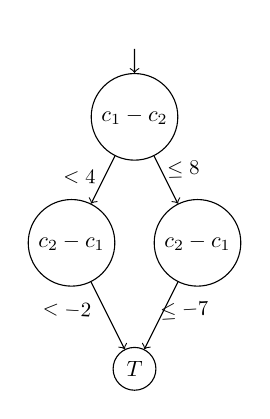
\begin{tikzpicture}[
		smallvertex/.style={circle,draw,scale=0.8}
		]
		\node[smallvertex](S0){$c_1 - c_2$};
		\node[smallvertex, draw = none, above of = S0, yshift = 0.25cm](S4){};
		\draw[->] (S4) --(S0) node [midway, above, sloped, scale=0.75,
		rotate=295, xshift =-0.4 cm, yshift = -0.2cm]{};
		\node[smallvertex, below of = S0, yshift = -1 cm, xshift = -1 cm](S1){$c_2 - c_1$};
		\node[smallvertex, below of = S0, yshift = -1 cm, xshift = 1  cm](S2){$c_2 - c_1$};
		\draw[->] (S0) --(S1) node [midway, above, sloped, scale=0.75,
		rotate=295, xshift =-0.4 cm, yshift = -0.2cm]{$<4$};
		\draw[->] (S0) --(S2) node [midway, above, sloped, scale=0.75,
		rotate=65, xshift =0.3 cm, yshift = -0.1cm]{$\leq 8$};
		\node[smallvertex, below of = S0, yshift = -3cm](S3){$T$};
		\draw[->] (S1) --(S3) node [midway, above, sloped, scale=0.75,
		rotate=60, xshift =-0.7 cm, yshift = -0.2cm]{$<-2$};
		\draw[->] (S2) --(S3) node [midway, above, sloped, scale=0.75,
		rotate=300, xshift =0.4 cm, yshift = -0.2cm]{$\leq-7$};
	\end{tikzpicture}
	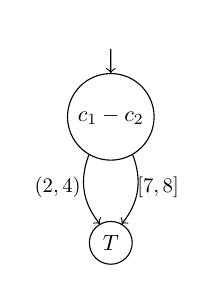
\begin{tikzpicture}[
		smallvertex/.style={circle,draw,scale=0.8}
		]
			
		\node[smallvertex](S0){$c_1 - c_2$};
	    \node[smallvertex, draw = none, above of = S0, yshift = 0.25cm](S4){};
		\draw[->] (S4) --(S0) node [midway, above, sloped, scale=0.75,
		rotate=295, xshift =-0.4 cm, yshift = -0.2cm]{};
		\node[smallvertex, below of = S0, yshift = -1cm](S3){$T$};
		\draw[->] (S0) edge [bend left](S3) node [midway, above, sloped, scale=0.75,
		rotate=0, xshift =-0.9 cm, yshift = -1.5cm]{$(2,4)$};
		\draw[->] (S0) edge [bend right](S3) node [midway, above, sloped, scale=0.75,
		rotate=0, xshift =0.8 cm, yshift = -1.5cm]{$[7,8]$};
	\end{tikzpicture}	
	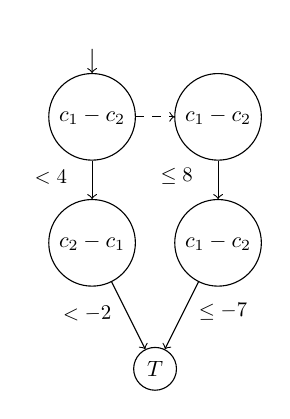
\begin{tikzpicture}[
		smallvertex/.style={circle,draw,scale=0.8}
		]
			
		\node[smallvertex](S0){$c_1 - c_2$};
		\node[smallvertex, draw = none, above of = S0, yshift = 0.25cm](S5){};
		\draw[->] (S5) --(S0) node [midway, above, sloped, scale=0.75,
		rotate=295, xshift =-0.4 cm, yshift = -0.2cm]{};
		\node[smallvertex, right of = S0, xshift = 1cm](S1){$c_1 - c_2$};
		\draw[dashed,->] (S0) --(S1) node [midway, above, sloped, scale=0.75,
		rotate=0, xshift =-0.7 cm, yshift = -0.2cm]{};
		\node[smallvertex, below of = S0, yshift = -1cm](S2){$c_2 - c_1$};
		\draw[->] (S0) --(S2) node [midway, above, sloped, scale=0.75,
		rotate=90, xshift =-0.7 cm, yshift = -0.2cm]{$< 4$};
		\node[smallvertex, below of = S1, yshift = -1cm](S3){$c_1 - c_2$};
		\draw[->] (S1) --(S3) node [midway, above, sloped, scale=0.75,
		rotate=90, xshift =-0.7 cm, yshift = -0.2cm]{$\leq 8$};
		\node[smallvertex, below of = S0, xshift = 1cm, yshift = -3cm](S4){$T$};
		\draw[->] (S2) --(S4) node [midway, above, sloped, scale=0.75,
		rotate=65, xshift =-0.7 cm, yshift = -0.2cm]{$<-2$};
		\draw[->] (S3) --(S4) node [midway, above, sloped, scale=0.75,
		rotate=297, xshift =0.7 cm, yshift = -0.2cm]{$\leq-7$};
	\end{tikzpicture}
	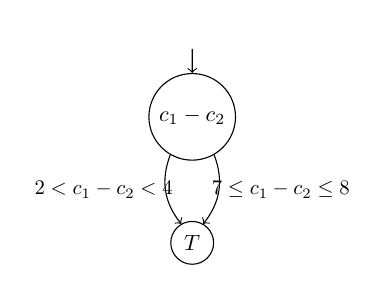
\begin{tikzpicture}[
		smallvertex/.style={circle,draw,scale=0.8}
		]
			
		\node[smallvertex](S0){$c_1 - c_2$};
		\node[smallvertex, draw = none, above of = S0, yshift = 0.25cm](S4){};
		\draw[->] (S4) --(S0) node [midway, above, sloped, scale=0.75,
		rotate=295, xshift =-0.4 cm, yshift = -0.2cm]{};
		\node[smallvertex, below of = S0, yshift = -1cm](S3){$T$};
		\draw[->] (S0) edge [bend left](S3) node [midway, above, sloped, scale=0.75,
		rotate=0, xshift =-1.5 cm, yshift = -1.5cm]{$2<c_1-c_2<4$};
		\draw[->] (S0) edge [bend right](S3) node [midway, above, sloped, scale=0.75,
		rotate=0, xshift =1.5 cm, yshift = -1.5cm]{$7\leq c_1-c_2\leq8$};
	\end{tikzpicture}	
	
\end{center}
\caption{A CRD, CDD, DDD and CMD representation}
\label{fig:examples}
\end{figure}

\begin{table}[]
\centering
\caption{Comparing Diagrams}
\label{table:diagrams}
\begin{tabular}{|l|l|l|}
\hline
Type                                                   & Pro                                                                                                                                                                                                                             & Con                                                                                                                                                                                                                                                          \\ \hline
DBM                                                    & \begin{tabular}[c]{@{}l@{}}Canonical form for convex zones\\ Existing library\\ Inclusion check\end{tabular}                                                                                                                    & \begin{tabular}[c]{@{}l@{}}Concave zones need multiple DBMs\\ Not memory efficient\end{tabular}                                                                                                                                                              \\ \hline
DDD                                                    & \begin{tabular}[c]{@{}l@{}}Structure like LDD\\ Re-ordering of variables possible\\ Apply same efficiency as BDDs\\ Boolean variables also in DDD\end{tabular}                                                                  & \begin{tabular}[c]{@{}l@{}}Canonicity hard to obtain\\ No on the fly canonicity\\ Expensive normal form computation\\ Only time performance tested\\ Only reduction algorithms\end{tabular}                                                                  \\ \hline
CDD                                                    & \begin{tabular}[c]{@{}l@{}}Structure like MDD\\ Inclusion check\\ (intersection of complement)\end{tabular}                                                                                                                     & \begin{tabular}[c]{@{}l@{}}No algorithm to get normal form\\ Only high level algorithms given\\ Methods don't maintain disjointness\\ Expensive normal form computation\\ No implementation results available\\ Disjointness memory inefficient\end{tabular} \\ \hline
CRD                                                    & \begin{tabular}[c]{@{}l@{}}Combination with BDD possible\\ Variable reordering shows advantage\\ Library available\\ Some benchmarks exp better than CDD\\ Extensive benchmarks\\ Good performance backwards reach\end{tabular} & \begin{tabular}[c]{@{}l@{}}3 possible canonical forms\\ No algorithms in paper\\ Some benchmarks linear worse than CDD\end{tabular}                                                                                                                          \\ \hline
CMD                                                    & Benchmarks against RED and UPPAAL                                                                                                                                                                                               & \begin{tabular}[c]{@{}l@{}}Results differ per case\\ Needs translation from vector to edges\\ Two reduced forms\end{tabular}                                                                                                                                 \\ \hline
\begin{tabular}[c]{@{}l@{}}BDD\\ discrete\end{tabular} & \begin{tabular}[c]{@{}l@{}}Using existing BDD packages\\ Good performance for small clock values\end{tabular}                                                                                                                   & \begin{tabular}[c]{@{}l@{}}Performance decreases fast for large values\\ Not possible with current opaal PINS\\ Introducing additional 'tick' actions\\ Only for closed timed automata\end{tabular}                                                          \\ \hline
\begin{tabular}[c]{@{}l@{}}BDD\\ zones\end{tabular}    & \begin{tabular}[c]{@{}l@{}}Using existing BDD packages\\ All variable reorderings possible\\ Only need direct translation DBM to\\ state vector\\ Easy to implement\end{tabular}                                                & \begin{tabular}[c]{@{}l@{}}Losing zone containment\\ No implementation results\end{tabular}                                                                                                                                                                  \\ \hline
\end{tabular}
\end{table}

A known difficulty in BDDs is the variable ordering. A bad ordering can lead to a BDD exponential in size where a good ordering can sometimes lead to a significant smaller diagram. Of the diagrams named above only CRDs have experimented with different orderings, the other researches assume a given ordering on the variables and the ordering of the values is fixed. The CRD case shows that full interleaving and having related variables close to each other in the ordering is preferable and gives the best results, both on speed and memory. This is the same result as expected with BDDs, this suggests that similar orderings should be used with these techniques.

\begin{figure}[t] 
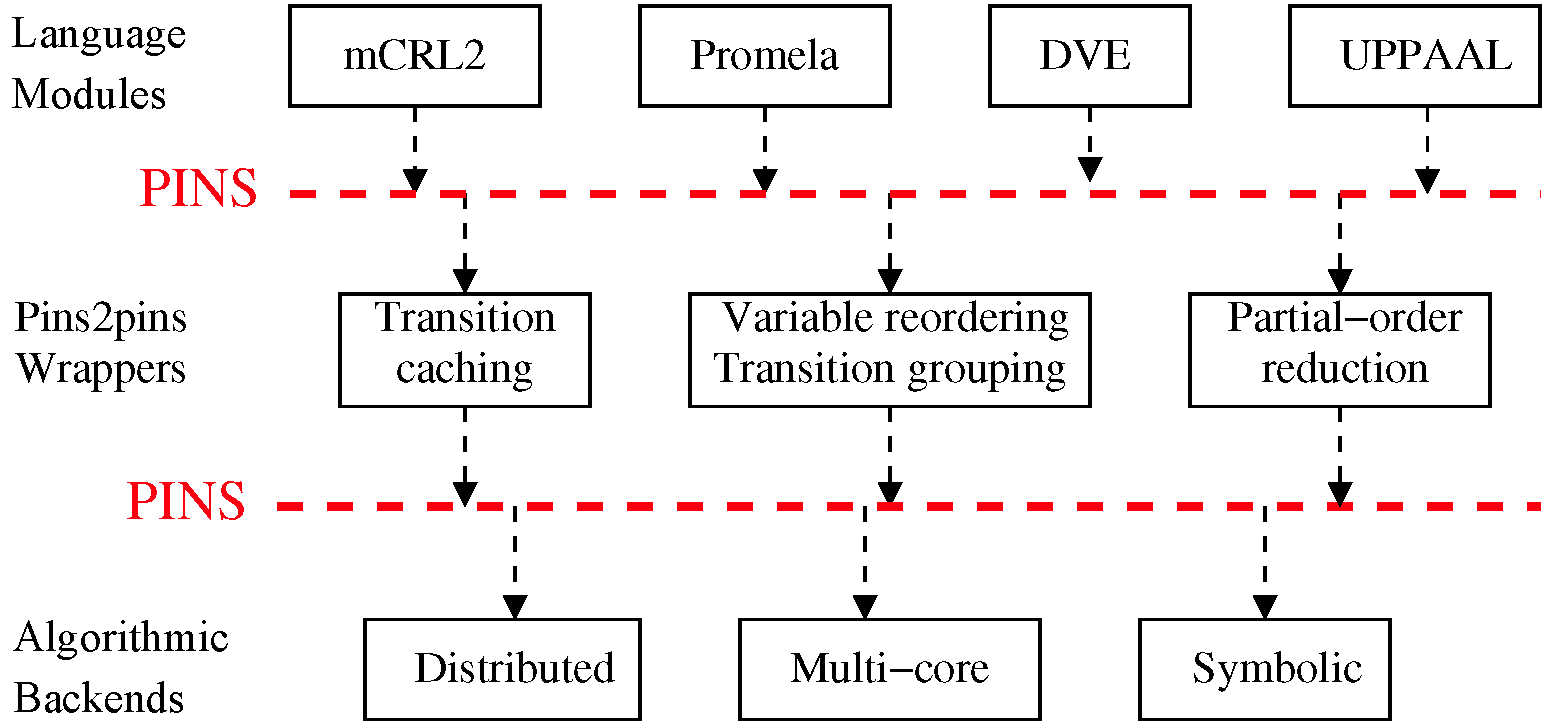
\includegraphics[width=\textwidth]{pins_modern}
\caption{Modular structure of LTSmin}
\label{fig:pins_modern}
\end{figure}

LTSmin~\cite{eemcs18152,ltsmin-mc:nmf2011} is a language independent model checker. It is build in a modular way such that new languages can be added by an PINS interface without too much effort, and new algorithms can be added more easily. LTSmin offers four different algorithmic back ends for model analysis: symbolic, multi-core, sequential and distributed. All of these back ends support different types of reduction and model checking. Several language modules have already been built for LTSmin such as mCRL2, Promela, DVE and UPPAAL. The modular structure of LTSmin is shown in figure \ref{fig:pins_modern}. States are stored in fixed length integer arrays. The PINS(Partitioned Next-State Interface) is the core of LTSmin. This interface abstracts as much as possible from the model without losing the structure. The main function of the interface is a (partitioned) next state function which returns the successor states. With these functions a state space can be generated on the fly. With the use of dependency matrices event locality can be determined statically~\cite{rwcmatrices}. Using these matrices, more efficient symbolic algorithms can be used, the number of next-state calls can be reduced and transition caching can be used. In the current UPPAAL PINS the next-state function is not partitioned and therefore no meaningful dependency matrix is created, and all of these algorithms can not be used.

\subsection{Timed Automata}
Timed Automata is a formalism that extends labelled transition systems with one ore more, but finite, clocks. As our work continues on ~\cite{eemcs21972} we use the same definition of timed automata.
\begin{mydef}[Timed Automata]
\label{def:TA}
An extended timed automaton is a 7-tuple A = $<L, C, Act, s_0, \rightarrow, I_c>$ where
{\renewcommand\labelitemi{--}
	\begin{itemize}
		\item L is a finite set of locations, typically denoted by $l$
		\item C is ia finite set of clocks, typically denoted by c
		\item Act is a finite set of actions
		\item $s_0 \in$ L is the initial location
		\item $\rightarrow \subseteq L \times G(C) \times Act \times 2^C \times L$ is the (non-deterministic) transition relation. We noramlly write l $\stackrel{g,a,r}{\longrightarrow}$ l' for a transition., where l is the source location, g is the guard over the clocks, a is the action, and r is the set of clocks reset.
		\item $I_C : L \rightarrow G(C)$ is a function mapping locations to downwards closed clock invariants.
	\end{itemize}
}
\end{mydef}

With this definition we can combine timed automata to a network of timed automata to define larger systems.

\begin{mydef}[Network of timed automata~\cite{eemcs21972}]
\label{def:networkTA}
Let Act = $\{ch!,ch?|ch \in Chan\} \cup \{\tau\}$ be a finite set of actions, and let C be a finite set of clocks. Then the parallel composition of extended timed automata $A_i = (L_i, C, Act, S^i_0, \rightarrow_{i}, I^i_C)$ for all $1 \leq i \leq n$, where $n \in \mathbb{N}$, is a network of timed automata, denoted $A = A_1||A_2||..||A_n$.
\end{mydef}

\subsection{Zones}
For basic transition systems the state space can grow exponentially for the size of the system. For Timed Automata the growth can become even larger and in some cases become unbounded by the addition of clocks. To tackle this problem most model checkers use a notion of zones for the representation of time. A zone can be seen as a set of constraints over the clocks C of the form $c_i \sim x$ and $c_i - c_j \sim x$ where $\sim  \in \{<, \leq, =, \geq, >\}$ and $x \in \mathbb{N}$. To represent these zones several data structures have been developed. One of the most common used structures are Difference Bound Matrices(DBMs)~\cite{dbmorig,bengtsson2002clocks}.
 
These matrices use both a column and a row for each clock, and on each position $(i,j)$ an upper bound on the difference between the clocks $c_i$ and $c_j$ is given in the form $c_i - c_j \preceq x$ where $\preceq \in \{<, \leq\}$ and $x \in \mathbb{N}$. For the constraints over the single clocks an extra clock $\mathbf{O}$ with a constant value 0 is added. By switching the two variables also a lower bound can be given to each pair. This way convex zones of clock variables can be represented. Each matrix can however only contain a single convex zone. Concave zones and multiple convex zones need multiple matrices to be represented. As a solution often a list of DBMs is used. 

\subsection{Difference Decision Diagrams}

We have discussed several symbolic approaches for representing zones. All of these approaches have benefits and downsides over each other. We chose to develop one of these approaches in LTSmin. The DDD approach has been chosen for this. It is a diagram form that is closely related to LDDs, for which we already have a library, and it is also quite compatible to the current PINS structure and its' next state function. The method still has some loose ends that need research, mostly on the algorithms and efficiently creating a canonical form. No results on the memory usage are available, which is normally the greatest benefit of a symbolic approach. So DDDs are a diagram type that seems to fit well in the current structure we have, but there is still room for some more research.

\begin{mydef}[Difference Decision Diagram~\cite{ddds}]
\label{def:DDD}
A difference decision diagram (DDD) is a directed acyclic graph $(V,E)$. The vertex set $V$ contains two terminals $0$ and $1$ with out-degree zero, and a set of non-terminal vertices with out-degree two and the following attributes.
\\\\
\begin{tabular}{lll}
Attribute                & Type                      & Description                                           \\\hline
pos(v), neg(v)           & \textbf{Var}              & Positive variable $x_i$, and negative variable $x_j$. \\
op(v)                    & \{\textless, $\leq\}$     & Operator \textless or $\leq$.                         \\
const(v)                 & $\mathbb{D}$              & Constant c.                                           \\
high(v), low(v)          & $V$                       & High-branch h, and low-branch l.                   
\end{tabular}
\captionof*{table}{}  
The set E contains the edges $(v,low(v))$ and $(v, high(v))$, where $v \in V$ is a non-terminal vertex.
\end{mydef}

In ~\cite{ddds} a canonical form for DDDs is discussed, also called a fully reduced DDD. Only definitions are given here, no algorithms to reach this form. It is stated that it is difficult to reach this fully reduced form. It is not clear if they managed to make their apply function in such a way that it maintains canonicity. To reach canonicity, local reductions and ordering are a first step, but it is not enough due to dependencies among the constraints. For BDDs the local reductions and ordering are sufficient to reach a canonical form. First we give some notational shorthands and then we define an ordering and local reductions on DDDs.
%
\begin{center}
\begin{tabular}{lll}
$var(v)$   & $=$ & $(pos(v),neg(v))$   \\
$bound(v)$ & $=$ & $(const(v),op(v))$  \\
$cstr(v)$  & $=$ & $(var(v),bound(v))$
\end{tabular}
\end{center}

\begin{mydef}[Ordered DDD~\cite{ddds}]
\label{def:ODDD}
An ordered DDD (ODDD) is a DDD where each non-terminal vertex $v$ satisfies:
\begin{enumerate}
  \item $neg(v) \prec pos(v)$,
  \item $var(v) \prec var(high(v))$,
  \item $var(v) \prec var(low(v))$ or \\ $var(v) = var(low(v))$ and $bound(v) \prec bound(low(v))$.
\end{enumerate}
\end{mydef}

After ordering a DDD some local reductions can be defined to reduce the size of a DDD.

\begin{mydef}[Locally Reduced DDD~\cite{ddds}]
A locally reduced DDD ($R_LDDD$) is an ODDD satisfying, for all non-terminals u and v:
\begin{enumerate}
  \item $\mathbb{D} = \mathbb{Z}$ implies $op(v) = '\leq'$,
  \item $(cstr(u),high(u),low(u)) = (cstr(v),high(v),low(v))$ implies $u = v$,
  \item $low(v) \neq high(v)$,
  \item $var(v) = var(low(v))$ implies $high(v) \neq high(low(v))$.
\end{enumerate}
\end{mydef}

These reductions are not enough to reach a canonical form. Here we define the other reductions and methods needed to reach a canonical form.

\begin{mydef}[Path-reduced DDD~\cite{ddds}]
A path-reduced DDD ($R_PDDD$) is a locally reduced DDD where all paths are feasible.
\end{mydef}

\begin{mydef}[Tightness~\cite{ddds}]
A dominating constraint $\alpha = x_i - x_j \lesssim c$ is tight in a feasible path $[p] = [p_1] \wedge \alpha \wedge [p_2]$ if for all tighter constraints $(c', \lesssim') < (c,\lesssim),$ the systems $[p_1] \wedge (x_i - x_j \lesssim' c') \wedge [p_2]$ and $[p]$ have different solutions. A path $p$ is tight if it is feasible and all dominating constraints on it are tight. An $R_LDDD u$ is tight if all paths from $u$ are tight. 
\end{mydef}

\begin{mydef}[Saturation~\cite{ddds}]
A tight path $p$ from an $R_PDDD$ is saturated if for all constraints $\alpha$ not on $p$, if $\alpha$ is added to $p$ either (1) $\alpha$ is not dominating and tight, or (2) the constraint system $[p_1] \wedge \neg\alpha$ is infeasible when $[p]$ is written $[p] = [p_1] \wedge [p_2]$ with all constraints on $p_1$ smaller than $\alpha$ with respect to $\prec$ and all constraints on $p_2$ larger than $\alpha$. An $R_PDDD$ $u$ is saturated if all paths from $u$ are saturated.
\end{mydef}

\begin{mydef}[Disjunctive vertex~\cite{ddds}]
Let $p$ be a path leading to the vertex $u$ in a DDD, and assume $\alpha = cstr(u), h = high(u),$ and $l = low(u)$. Then $u$ is disjunctive in $p$ if $[p] \wedge (\alpha \rightarrow h,l)$ and $[p] \wedge (h \vee l)$ have the same set of solutions.
\end{mydef}

All of these definitions lead to the following definition of a fully reduced DDD.
% 
\begin{mydef}[Fully reduced DDD~\cite{ddds}]
\label{def:RFDDD}
An $R_pDDD$ u is a fully-reduced DDD ($R_FDDD$) if it is tight, saturated and has no disjunctive vertices.
\end{mydef}

DDDs are also used to represent the discrete variables in automata. This is done by translating the variable into a difference constraint. For example $x_1 = 3$ will be translated into $x_1 - 0 \leq 3 \wedge 0 - x_1 \leq -3$, thus resulting into a DDD with two nodes. 

So far we only found the results of two benchmark tests of DDDs, Milner's scheduler and Fischer's protocol~\cite{Møller200253}. Here the DDD approach has been compared with KRONOS and UPPAAL which were both slower than the DDD implementation. The results of these benchmarks show no memory usage.  

\section{Plan}

\subsection{Questions}
For the research we will state a couple of research questions:
{\renewcommand\labelitemi{--}
	\begin{itemize}
		\item Is the combination of BDDs and flattened DBMs an efficient method for symbolic reachability analysis of timed automata? Both on memory usage and speed.
		\item Can improvements be achieved by using different orderings? Both by changing the order of only the clock variables and by mixing the clock and state variables.
		\item Is the new language module needed for the symbolic approach also usable for the multicore approach with subsumption?
		\item Can the BDD approach be generalized towards a method using DDDs?
		\item Can we create a fully symbolic reachability analysis for timed automata using DDDs, without using DBMs?
	\end{itemize}
}

\subsection{Zone Containment}
In BDDs it is simple to test for containment of a state. This can be done in linear time over the number of variables. For zones in DDDs this can be a harder question, as a zone can be contained in some larger zone in the DDD. For this we need an extension to the normal LDD algorithm, that can handle these zones. The main difference is that on some nodes both the high and the low edge can lead to a satisfying path. Algorithm \ref{alg:contain} tests if a zone $z$ is contained in the DDD rooted at $v$.

\begin{algorithm}
\caption{Zone containment for DDDs}\label{alg:contain}
\begin{algorithmic}[1]
\Procedure{Contains}{$v, z$}
	\If{$v \in {0,1}$} 
		\Return{$v$} 
	\EndIf
	\If{z[$var(v)$] correct in $v$}
		\If{\Call{Contains}{$high(v), z$}} 
			\Return{\True}
		\Else{ 
			\Return{\Call{Contains}{$low(v), z$}}} 
		\EndIf
	\Else{ 
		\Return{\Call{Contains}{$low(v), z$}}} 
	\EndIf
\EndProcedure
\end{algorithmic}
\end{algorithm}

Where the correct in check will evaluate if the upper-bound in the zone is lower than the upper bound in the node $v$. As we will use maximal sharing of subtrees, some nodes might be revisited. Once we revisit a node, we know that none of it subtrees will lead to a correct evaluation. Therefore we could use a visited flag, to save computation time. The worst case running time of the algorithm will be $\mathcal{O}(|v|)$, where $|v|$ is the number of nodes in the DDD. This can increase the running time of the state space generation significantly, as this algorithm will need to be ran every time a new state is found. It will however save memory, as no zones will be added that are already in the DDD. As the main goal of a symbolic approach is the reduction of memory, we think this is the better solution, over a less time consuming approach which would lead to more memory consumption. The algorithm will not work correctly when the discrete variables are also translated into DDD nodes, as the value in those cases needs to be correct, and an higher upper bound will not work. For the mix of DDD and LDD nodes we will need to change the algorithm to algorithm \ref{alg:containLDD}. This algorithm checks if a node is of type DDD. If it is, the old algorithm will be executed normally, if not, then it is an LDD node and in case of a correct evaluation only the high edge will be explored. The low edge will in that case never lead to a correct evaluation of the state.

\begin{algorithm}
\begin{algorithmic}[1]
\caption{Zone containment for mixed diagram}\label{alg:containLDD}
\Procedure{Contains}{$v, z$}
	\If{$v \in {0,1}$} 
		\Return{$v$} 
	\EndIf
	\If{z[$var(v)$] correct in $v$}
		\If{$type(v)$ is DDD} 
			\If{\Call{Contains}{$high(v), z$}} 
				\Return{\True}
			\Else{ 
				\Return{\Call{Contains}{$low(v), z$}}} 
			\EndIf
		\Else{
			\Return{\Call{Contains}{$high(v), z$}}}
		\EndIf 
	\Else{ 
		\Return{\Call{Contains}{$low(v), z$}}} 
	\EndIf
\EndProcedure
\end{algorithmic}
\end{algorithm}

\begin{algorithm}
\begin{algorithmic}[1]
\caption{Union}\label{alg:union}
\Procedure{Union}{$v1, v2$}
	\If{$v1 = v2$} 
		\Return{$v1$} 
	\EndIf
	\If{$v1 =$ \False}
		\Return{$v2$}
	\EndIf
	\If{$v2 =$ \False}
		\Return{$v1$}
	\EndIf
	\If{$v1 \prec v2$}
		\State $high \gets$ \Call{Union}{$high(v1), high(v2)$}
		\State $low \gets$ \Call{Union}{$low(v1), v2$}
		\State $result \gets$ \Call{Mk}{$cstr(v1), high, low$}
	\EndIf
	\If{$v2 \prec v1$}
		\State $high \gets$ \Call{Union}{$high(v1), high(v2)$}
		\State $low \gets$ \Call{Union}{$v1, low(v2)$}
		\State $result \gets$ \Call{Mk}{$cstr(v2), high, low$}
	\EndIf
	\If{$v1 = v2$}
		\State $high(v1) \gets$ \Call{Union}{$high(v1), high(v2)$}
		\State $low(v1) \gets$ \Call{Union}{$low(v1), low(v2)$}
		\State $result \gets$ \Call{Mk}{$cstr(v1), high, low$}
	\EndIf
	\Return $result$
\EndProcedure
\end{algorithmic}
\end{algorithm}

\subsection{Approach}
We will propose first a method that will use the best of both worlds. We will use the DBMs in the state exploration such that we can find a canonical representation of the clock zone of a newly explored state quite easily. For the symbolic representation of the state space, including the clock zones, and the transition relations, we will use normal BDDs. The DBMs will be flattened and put directly into the state vector and can than be handled by the symbolic BDD backend. Therefore both the efficient algorithms and the memory efficient representation can be used. A downside to this approach is that a zone subsumption check is not possible anymore, resulting in revisiting of some states. Further we will focus on efficient orderings of the BDDs, as both clock zones and states are contained in a single structure. We will also use this new method with the existing multicore tool, such that we can still use the subsumption check. Afther that we will continue towards a DDD model checker. First we will use the DDDs as the state space representation and still use the language module using the DBMs. We have not been able to find any literature on the combination of these techniques. There might be a significant memory improvement possible here. Eventually we want a complete symbolic solution with more operations on the DDD, such as the progress of time, then we can have a language module which does not use the DBMs any more. We will compare this approach extensively to other approaches. All of these approaches will be implemented in the LTSmin toolset. This way we can really compare the methods and not just the tools.

Alongside this we will also have to make the opaal PINS work with the UPPAAL models generated by ANIMO. The current versions doe not work together because of global variables are used in the system declaration in the generated model. We can make this work by either changing the models generated by ANIMO or by extending the opaal PINS. At this time we do not know the best solution for this problem.

\subsection{To do}
In this section we describe all things that need to be implemented to make model checking with a certain diagram possible. 

To make symbolic model checking work we need to change the opaal PINS. The PINS currently uses a pointer to a DBM. For the new approach we will put the values of the DBM directly into the state vector. This will increase the size of the state vector. All other references to the types and values of the state vector entries will need to be changed also. 

To make symbolic variable reordering possible we will need to partition the next state function and create a dependency matrix. In the code the next state function is already split up per transition, but in a single transition group. Splitting this into multiple transition groups should not be too hard. In this same step also the dependency matrices need to be created and made as sparse as possible.

To combine the new PINS with the multicore LTSmin backend the subsumption check will need to be changed. This check now relies on a pointer to a DBM, but it will now get the complete DBM, or state vector. Here the search algorithm or the subsumption check will need to know which variables are zone variables. It will also occur that different states will have the same discrete variables, but different zone variables, these all need to be checked for the subsumption check.

For the combination with the multicore backend also the data structure will need to be adapted. The current structure stores a discrete state together with a set of pointers to DBMs. In the new situation each pair of discrete state and DBM will be stored explicitly.

For the DDD the diagram will need to be able to identify the zone variables from the discrete state variables in the state vector. This will need an extra function in the PINS interface recognizing the different types of variables.  

For the DDD representation the values from the DBM will need to be translated to useful variables as ordering of the DDD is based on the values. Also to check for inequalities and set containment the meaningful values are needed. In the current DBM library both the value and the operator are saved in a single 32 bit integer. The DDD will need to know the value and the operator separately.

To make an efficient DDD representation, we need to mix these DDD nodes with BDDs or LDDs for the discrete variables. For this diagram this has not been done before, we can only look at the CRD solution. Algorithms probably need some adaptation for these multiple types of nodes. Also the possibility and results of the mixing of discrete and zone variables need to be researched. It might be that it functions better when the two types of variables remain separated, or when they are mixed.

\subsection{Planning}
In the table below we have put all actions that need to be done into tasks. In the second column we put which tool should work correctly for the opaal language module after the task. This will give us intermediate points on which we can test the work that has been done to that point.

%\begin{table}[]
%\centering
%\caption{Tasks}
\label{table:tasks}
\label{my-label}
\begin{tabular}{@{}ll@{}}
\toprule
Task                                            & Needs to function                                                           \\ \midrule
Flatten the DBMs                                & Symbolic tool                                                               \\
Partition the next state function               & Symbolic tool                                                               \\
Create dependency matrices                      & \begin{tabular}[c]{@{}l@{}}Symbolic tool\\ variable reordering\end{tabular} \\
Change subsumption check for multicore approach &                                                                             \\
Other adaptions multicore approach              & Multicore tool                                                              \\
Create minimal DDD library                      &                                                                             \\
Combine DDD with LDD                            &                                                                             \\
Extend language module for DDD approach         & Symbolic tool                                                               \\
Benchmark tests for multiple approaches         &                                                                             \\
Test with ANIMO models                          &                                                                             \\
Extend DDD library for fully symbolic approach  &                                                                             \\
Change language module for fully symbolic DDDs  & Symbolic tool                                                               \\
Benchmark Testing fully symbolic approach       &                                                                             \\
Writing Report                                  &                                                                             \\ \bottomrule
\end{tabular}
%\end{table}

\bibliography{references}{}
\bibliographystyle{unsrt}
\end{document}